\Chapter{The Garden}{Clare Court}

Almost as soon as William and Ada had got themselves into the gaunt, bare shell of a house and installed their belongings, they began the task of making a piece of garden near the house - mainly a patch of orchard grass, which soon responded to cutting and became a very pleasant lawn. Garden making was quite a new experience for Ada, and as they began the tasks of making paths, and establishing beds of flowers, she very soon found herself in her element. For years she had been tied to the house across the road for all of her waking hours - counter work during the day while after hours she coped with all the whims and fancies of a domineering and not very sweet-tempered taskmistress. Suddenly she found herself in her element, and as the busy years slipped by she spent more and more time in the garden. It became a hobby and an amusing challenge to collect stones for rockeries and ornaments. Often on an evening walk she and William would see a stone which caught their fancy and laboriously carry it home between them. The cliffs at Watchet are veined with seams of alabaster which was an important factor in the establishment of the paper mill over two hundred years ago, alabaster being an important whitening agent in the manufacture of paper. The colours are many and varied, from rose and white to creamy yellow and green, and many pieces of alabaster found their way into the garden. Unfortunately, once it has been cut away from the cliff and left for a while in the open air, the delicate shades and sparkling crystals of the stone become quickly misted over and after a few years it becomes badly discoloured.

As the years went by and their business became established and relatively prosperous, William and Ada were able to afford more help with the shop and post office and this enabled them to spend more time in the garden.

At its heyday during the 1930s, our modest domain at Washford was a veritable little empire, with constant coming and going of postmen and customers throughout the day. William always employed at least one \quotemark{boy} to help with the repairs - sometimes he had grown to be a man while in the service but had usually started his employment with William on leaving school. Ada always had a girl in the office and one or two telephonists. One of William's dislikes was vegetable gardening, and he was only too happy to delegate entire charge of this part of the garden to Bert or Graham or Stan. Country boys all, they were usually wonderful gardeners, and never happier than when \quotemark{spitting} or burying the dung. William could occasionally be seen, in waistcoat and hat and bow tie, tastefully clipping the ornamental hedges into fanciful shapes. A great lover of the curved line, he did not care for his hedges to be straight along the top, and the nitida sported many simulated pillars surmounted by knobs and joined by graceful curved spans that would not have disgraced a gentleman's residence. Alas! In these utilitarian days, they are not a faint shadow of their former selves, but here and there an obstinate downward curve and drunken pillar leaning precariously to one side, wryly remind us of their departed elegance.

Ada on the contrary adored flower gardening, and this was her main relaxation, affording the principal outlet for her creative talent, not forgetting the crochet work of course. Unfortunately I never saw the garden at its peak. When I first came to Washford, old age and ill health were beginning to take their toll, and the ornamental rockeries had quite a few weeds in them. Out of self-preservation we have had to eliminate many of the smaller beds as it was quite impossible to keep them all tidy. One day when everything else is finished I hope to get the part that remains back to something approaching its former charm. One is speechless at William and Ada's industry as, at the same time that they were creating the garden, they were also running the business and Post Office, finishing the building of the house, bringing up a child and taking an active part in church and council work. It is perhaps hardly surprising that some things were never completed.
 
\Flourish	 

I have already mentioned Ada's rather naughty habit of acquiring stones for her garden. She need not have carried so many; ten years after the house was built they were to have far more than they could use when William demolished the two old cottages. An astonishing assortment emerged from the rubble - fragments of capitals, octagonal sections which must surely have been the vertebrae of columns, curved stones, square stones, rectangular stones - all these and more emerged from the masonry as the walls collapsed and the dust began to clear. The largest pieces were enormous and could only just be lifted by one man on his own. They stand around the garden at various points, silent memorials to the mediaeval masons who first quarried and sculpted them. I sometimes wonder what they were called, those masons of long ago. Were they Cridlands or Burnetts, Goodings, and Locks in the village In the Middle Ages? What did they talk about while they were shaping the soft red sandstone into those gently rounded curves or geometrical shapes? The success of the harvest, the monks at the new Abbey, and did they grumble about the taxes - or simply talk about the weather? The air is silent and there are some questions to which we shall never know the answer but six hundred years after the Abbey was first founded the stones continue to bear silent testimony to those long-dead craftsmen. Then again, the imagination flits over another period of time, to the 1560s, when the Abbey Church was pillaged after the Dissolution of the Monasteries. Were they descendants of those masons, who came along with their oxen and took away free cart loads of stone? It seems a miracle that the actual Abbey buildings still survive, but this part of the Abbey continued to be used as a farm and perhaps even as a place of residence and that is presumably why it was never allowed to fall into too bad a state of repair. Of the church, however, not one single stone remains. Patient excavation has revealed the shape and size of it, and the bases of the pillars are clearly to be seen. It must have been a magnificent sight in its prime - such a splendid building with its soaring nave and tower amidst the lush greenery of the valley. Monks always seem to have had a wonderful knack of finding the most sheltered and fertile spot in which to build their Abbeys. This well-watered vale, so effectively shielded from cold winds by its surrounding ring of hills, must surely be one of the gentlest nurseries for cultivating tender plants. One can easily imagine vineyards growing here in mediaeval times for it is known that the vine was cultivated in this area.

\begin{figure}[p]
	\centering
     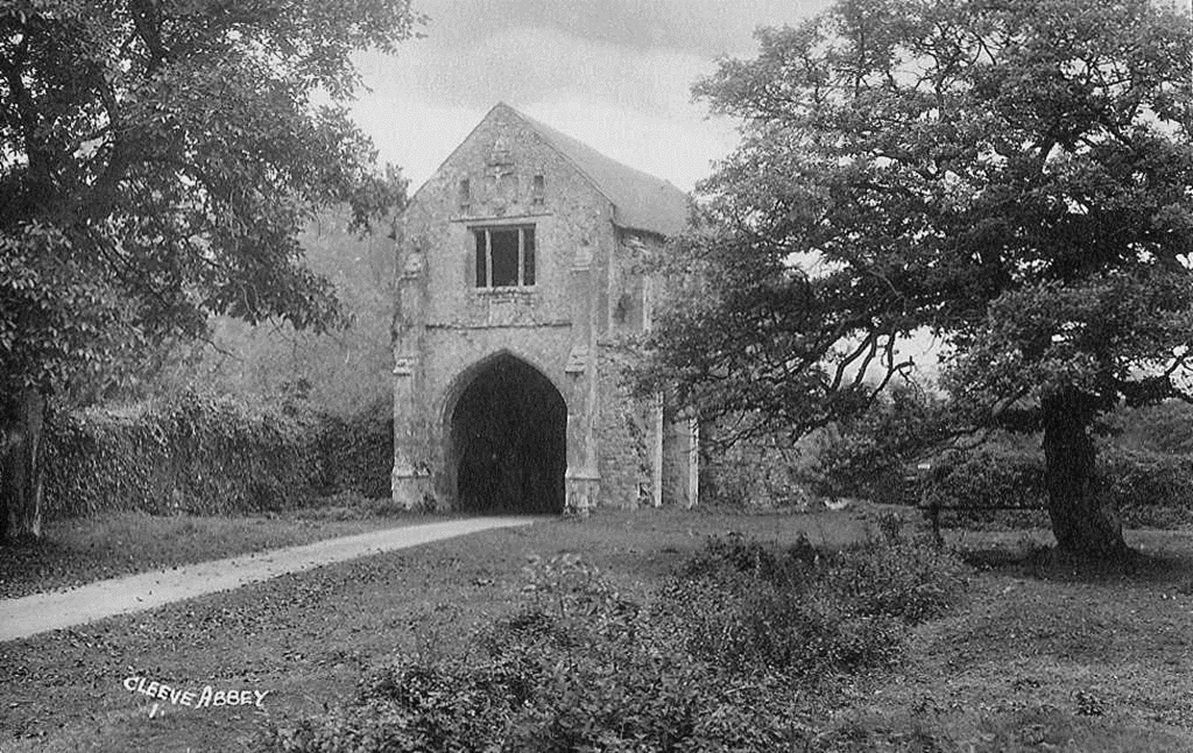
\includegraphics[width=1\textwidth]{figures/CleeveAbbey}
     \caption{Cleeve Abbey, Gateway}
     \label{fig:CleeveAbbey}
\end{figure}

\begin{figure}[p]
	\centering
     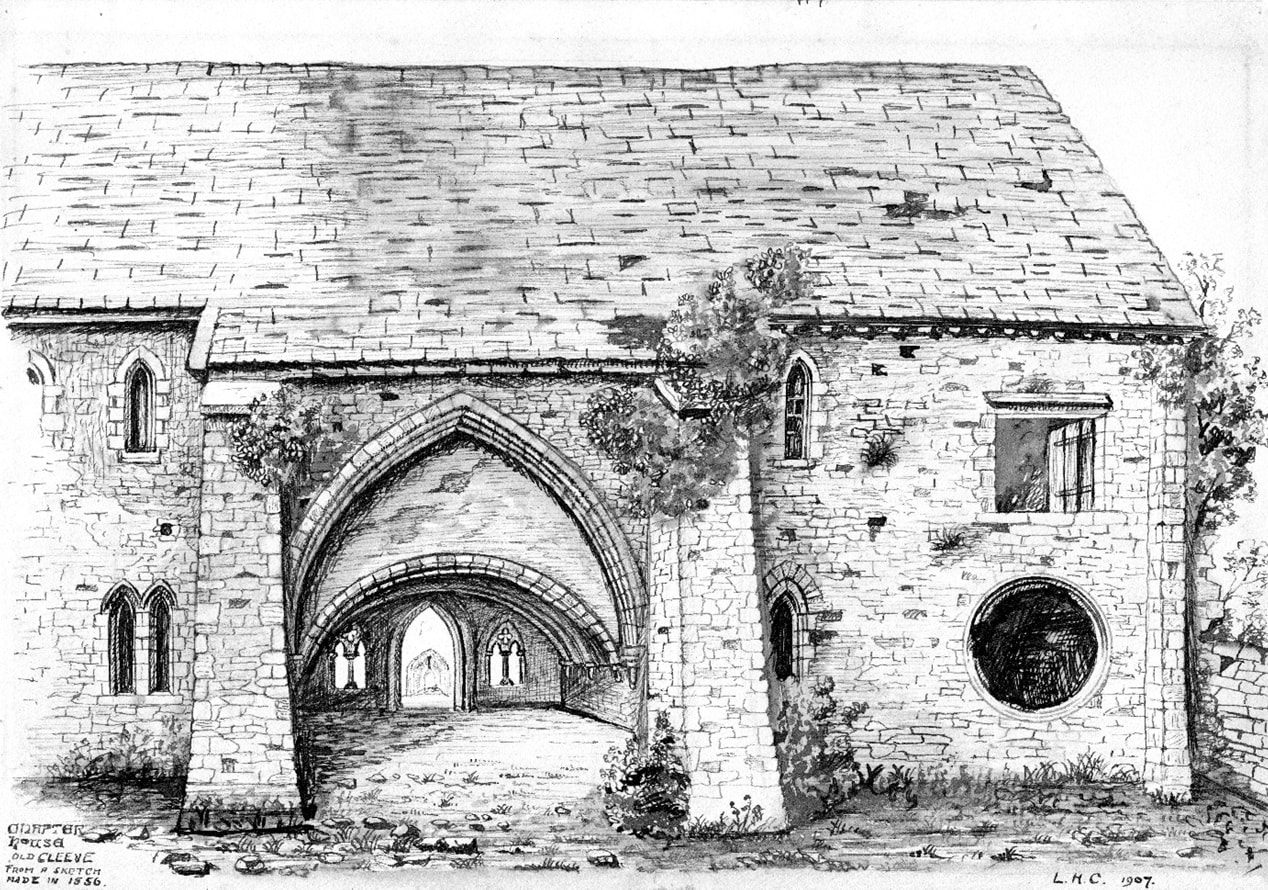
\includegraphics[width=1\textwidth]{figures/ChapterHouse}
     \caption{A sketch of Cleeve Abbey Chapter House made in 1856}
     \label{fig:ChapterHouse}
\end{figure}

\afterpage{\clearpage}

Before the supply of stones became so abundant the first paths and steps in the garden were made of the most readily available materials. Treborough slate, which figures prominently, was used to pave the principal paths. Slate has its disadvantages among which a tendency to become slippery in wet weather is the worst. However, we know our paths well and rarely slip on them ourselves. Some of the slabs are very large and thick, and the labour of moving them and putting them into place must have been enormous. One particularly splendid square piece which we have served for forty years or so as a base for the stamping pad in the post office. It is about two foot square and two inches thick - they evidently anticipated heavy use! It would not have been out of place as a chopping block. I have not yet found a use for it but no doubt the day will come.I am beginning to see the wisdom of the old country adage \quotemark{keep a thing for seven years and you'll find a use for it}!

% 14: Cleeve Abbey, Gateway
 
% 15: Cleeve Abbey Chapter House

To start the garden off then, they had a good piece of grass at the side and front of the house, and a few paths. Shortly afterwards they made some steps leading up from the lawn towards the wash house, and these have always been very successful as a background for family photographs. The paving was of red sandstone and finding it difficult no doubt to finish off the steps in the desired curve	with such an awkward material, William cast the ends of the steps himself in concrete which has mellowed over the years to blend with the natural stone. He was talented too at designing his garden ornaments and casting them in cement, and Benvenuto Cellini can hardly have had greater satisfaction at the unmoulding of Perseus than William at the production of his plant pots and ornamental plasters. The moulds for these lie around somewhere still. The cement he used must have been different from our modern variety as it has weathered to a pleasant greyish shade. Some of the steps have an almost glass-like smoothness - I am told that the materials for achieving this type of finish are not obtainable nowadays. When desiring to create a variation in the finished product he would set small pieces of alabaster broken up into the moulds, or occasionally pieces of sandstone in different shades. I enjoy putting plants in these pots but alas! I lead a busy life and am frequently prone to forget them, upon which the unfortunate occupants languish and die. One thing is certain - I could never introduce factory made ornaments into our garden to stand beside those that we have - although quite pleasant in appearance, the contrast would be hopelessly incongruous.

Besides the steps there are two hollow pillars made by the broken alabaster mould method surmounted by two more pots. He also constructed two steps to the lower level of the garden which was later to contain the pond. The pillars beside these were made of old bricks in order to achieve a more attractive appearance, and William painstakingly chipped the edges from each individual brick. These pillars are hollow, which tempts garden birds to build their nests inside. Unfortunately our two cats are only too aware of their presence and despite our efforts to protect the squatting family of baby sparrows this spring, the mother abandoned the nest in the face of such energetic feline interest. Even when there is nothing inside the pillar, it is not an uncommon sight to see a cat's tail protruding from the top - our adventurous and agile cat likes to know what is at the bottom and we often wonder if she will succeed in getting herself out again. Rather to our surprise she generally manages the feat unaided.

All the lower part of the garden would have been made during the 1930s after the two old cottages had been knocked down, and one is continually amazed at the achievement considering the nature of the times. From about 1930 onwards the villages were hit very hard by the depression. The majority of the village population was living on a very low income, and many on the five shilling per week unemployment benefit. Takings in the shop dropped to a pathetically low level, just sufficient to live on with little or nothing left over to pay back the heavy interest charges to the bank. For years money was in such short supply that every possible expedient was resorted to in order to manage without it. And yet throughout this time, William and Ada never stopped working in the garden, creating charm and even beauty from materials that were readily to hand and which cost little or nothing. As far as the actual plants were concerned stocking the garden was very much a family affair. Flora Thompson in \quotemark{Lark Rise} describes how cottagers in the 1880's lovingly tended their plots and filled their tiny gardens with clumps of cottage flowers, which they acquired by exchanging with each other. Country folk of the labouring class rarely had pence to spare from their low wages to buy seeds, and so it was, indeed still is, common friendly practice to give a neighbour a slip of an admired plant. Ada continued the tradition and nothing gave her greater delight than to acquire a new cutting or give a home to a languishing plant. Her favourite birthday or Christmas gift would be a rose tree to augment her collection. Unfortunately I do not know the origin of those that survive of the eighty bushes which she once counted in her garden. Some of them are very old to judge by their stems, and of varieties rarely seen nowadays, so perhaps they are a legacy from the pre-1914 cottage garden. The blooms are smaller and nearer to hedge roses in style and colour than the enormous waxy monsters to which we have become accustomed. One in particular which I estimate to be at least forty years old is of a very unusual pinky mauve shade. Sad to relate, during the fifties and sixties when the upkeep of the garden was becoming increasingly difficult, Ada discovered chemical weed killers, and not understanding the danger in using them poured large quantities of sodium chlorate solution over the paths. The inevitable result which never failed to surprise her was that many plants disappeared, never to be seen again. Several ornamental trees were also severely affected and branches died on the almond and cherry trees. It has taken several years for the garden to recover from this chemical assault and we have partly nursed the sick trees back to health. Although their shape is ruined, it is nice to keep some trees from the original garden, however imperfect they may be - especially when one remembers the loving care and devotion with which they were raised, sometimes from a pip or stone.

Ada was in a more fortunate position than her labouring ancestors when it came to obtaining flower and vegetable seed as William held the agency in the village for Webbs seeds. In those days when there was still a strict code of honour prevailing among wholesalers and their customers in the villages, the agency to such a firm was a valuable asset not to be lightly dismissed. If you were the sole agent then you knew that you really were the only shop to be selling that particular brand of goods and would never suffer the annoyance which we had to endure when we tried to run the shop for a while of seeing another shop in the village selling goods which were traditionally our preserve. That sort of integrity is hard to maintain in these competitive days, but its loss was a sad day and drove one more nail into the coffin of the spirit of mutual trust and confidence which used to prevail between traders in the same community. In the early days the seeds used to arrive by train in strong, pleasant looking wooden boxes - we have two or three of them still, and the one in which I keep my spare cutlery does not look out of place near the polished oak under the hall stairs. Ada was as proud of Webbs seeds as if she had ripened and harvested them herself and many a bed of cornflowers, stocks, nasturtiums and candytuft flourished under her care. She was not a very methodical gardener and I never remember her raising seedlings and transplanting them into pots when they showed two leaves and all that sort of thing. She just had green fingers and her constant vigilance - for she thought nothing of going out in the garden after sorting the morning mail for a couple of hours before breakfast, which she herself did not eat and in the long summer days was quite likely to be still out until darkness came in at around ten o' clock - ensured that the seedlings were not eaten by slugs or smothered by weeds. As already mentioned she was an inveterate pip planter and as she grew older the pots on the window sill became one of her principal interests. After her death there was a fine little orange tree and several budding date palms on the sill of the larder window, but I am afraid in the chaos that prevailed for the first year of running two homes and shuttling to and fro between them, the plants were neglected and suffered an untimely death.

The tradition of window sill gardening seems to be very old among country people and it is one of the most delightful characteristics of the English village scene. To me it seems a small miracle that when the production of food occupied such a large and important part of their lives, cottagers always managed to find a corner for a clump of phlox, sweet rocket and a briar rose as well as the sweet smelling and decorative herbs, rosemary, thyme and sage. The window sills (or sill) were a valuable extension of the often tiny garden as contrary to general belief many cottagers have virtually no garden at all. Fashions in window sill gardening do not change very rapidly and it still a fairly common sight in these country parts to see a maidenhair fern or Mind-your-own business overflowing a Victorian plant pot decorated in those rather vivid shades of green and pink so beloved of our grandparents. It was pleasant too to see, when a group of modern bungalows was built in our village for older residents, that it was literally no time at all before the windows, much larger than any most of the occupants had ever owned before, boasted a delightful display of Busy Lizzies, Christmas Cactus, scented geranium, and other traditional cottage flowers, as well as the more modern varieties of gloxinias, begonia and primulas. The only nation to outdo the English cottager in this respect must surely be the Dutch - to drive along a street of tiny bungalows almost anywhere in Holland is like visiting a florist's display, so crammed is every available inch with a wealth of leaf and bloom, climbing vine and trailing fern.

Gradually then, the garden took shape, with a stone added here, a cutting there, a seedling oak tree raised from an acorn in the hedge, and tell it not in Gath, more than one mysterious stranger which somehow accidentally found its way there by way of Ada’s handbag after a visit to a park or garden. What a strange malady it is which seems to afflict many gardeners who are scrupulously honest in every other way - the burning desire to break off a small piece of a plant which catches their fancy! It is a disease which cuts right across class and social status and I confess that I myself am not totally immune from it. There seems to be a rough moral justice being meted out from above as somehow or other these \quotemark{acquired} cuttings rarely seem to grow.

After the demolition of the cottages there was such a large quantity of stones to dispose of that it took years to \quotemark{find a use} for all of them and it must be confessed that the main use for a large quantity of them was to provide a convenient home for snails and weeds. Over the years we have gradually put together the evidence together with what Glyn can remember, and the analysis makes an interesting study of the old country philosophy that nothing must ever be thrown away. Take the stones to start with - I have already described the uses to which the best ones were put, steps, building walls, ornamental pillars and a simulated well, incorporating the curved stones from the pillars of the former church. Selecting some of the square blocks, William even took the trouble to make a mounting block, chipping out a date and incorporating it into the stonework. I am sorry to say that most of the block has been submerged by the car park and only the top slab is now visible. It would not be too difficult to dig out the stones and reconstruct it somewhere else and perhaps one day the money will be found to have this done. Needless to say, it was never used as a mounting block- I doubt whether Ada got on horseback in her life. Grandfather William had always kept a pony and was a well-known sight riding to services and meetings, so William had learned to ride. But he discovered the internal combustion engine at an early stage and bought one of the first motor cycles to be seen in the district - a 1913 \quotemark{James} (Figure \ref{fig:James}). We still have it.

Of the vast surplus of stones remaining, many little rockeries and walls with little paths intertwining were constructed. Quite a large number were used to raise the level of the path leading out to the road - since the raising of the main thoroughfare all the paths and gates had had to be altered and there were steps up to the road. We discovered masses of these buried stones when digging a trench for a new drain - it certainly did not make for very rapid progress as each one had to be prised out individually and lifted out by hand. These were the very rough stones in their natural state as they would have left the quarry in the thirteenth century - the infilling of the massive walls of the Abbey Church.

One cannot help thinking that by far the best solution would have been to get rid of the rubble in some way - invite farmers to take the stones to tip in gateways and that sort of thing. It would certainly have saved a great many headaches and backaches in later years. However, these were not William's methods! The very idea of actually getting rid of something that was not only necessary, but actually an encumbrance, was utterly foreign to their philosophy. Having left behind them the century when working folk had few, if any possessions apart from the bare necessities of life, they had not re-adjusted to the dawning of our disposable, pre-packaged, throwaway age. There is little doubt that already the problem of refuse disposal was beginning to be felt for there were no regular rubbish collections in those days. Many of the items which had to be buried in the garden were symbolic of the motor age which was getting well under way and leaving its mark even in rural corners such as ours. A neighbour tells us that the top of the garden has had just about everything imaginable thrown on to it, including a large quantity of old car oil, acid from batteries, not to mention the batteries themselves, all of which we now know finds its way into the water supply and pollutes our rivers. Pollution was a word unknown to them - William and Ada would have been quite put out if anyone had pointed out to them that they were harming the environment by these and similar activities such as the lavish use of weedkiller. It has taken writers such as Rachel Carson to awaken us to the true horror of these problems - yet still one can walk into a hardware store and buy enough deadly poison (disguised as sodium chlorite or paraquat) to kill off the entire population of Washford.

Sometime in the early 1930s William and Ada had been to a sale at Wedmore and acquired very cheaply a large quantity of second hand materials. This sale was often mentioned and I think: that it must have been a big event in William's life. I used to wonder why they spoke of it so often, but as Wedmore is at the other end of Somerset and they never went away on holiday until well into the 30s it is not difficult to see that a journey to a completely unknown town was quite an exciting excursion. Having got to Wedmore he evidently considered that the greatest possible value should be extracted from the visit and bought a large quantity of stained glass. Several of the doors and windows in the house were subsequently made to fit round the glass and some of it was even used to beautify the door of the Toe H. Other panels never found a use and lay around in the corners of outbuildings along -with the oak Grandfather’s sewing machine, the globes and (mostly; old crates and rubbish. One pair of glass panels in particular must have caught Ada's fancy as she kept them in her bedroom. They depict knights in armour apparently keeping vigil, and at a casual glance one might think that they are old, but the expression on the faces of the knights is so righteous as to be comical. I can only guess that they were panels in the door of some large Pugin-type Victorian residence which was being demolished.

What else have we which was created from all this spare material? Stones, bricks - gradually, laboriously and with an infinite amount of heavy physical labour these were dispersed. Then there were the red quarry tiles from the cottage floors, of a thickness undreamt of nowadays! How surprised our grandfathers would have been to see us bring home a few cardboard boxes from the hardware shop and stick down a whole floorful of tiles in a mere matter of hours. These quarry tiles measure eight and a half inches square and are an inch and a half thick. They are of a pleasant mellow brick-red shade and have lain now fully exposed to the elements for forty years or so without suffering any apparent deterioration. They make a pleasing path around the summer house and also finish off the top of one or two of the ornamental pillars. They must be strong; as only last evening, one of our cats jumped up rather suddenly and to her great surprise knocked one of them sharply to the ground. The cat was very surprised at the sudden disappearance of her perch but despite the sharp bump the tile did not break.

Surely I must have nearly finished the catalogue of re-usable materials from this pair of apparently very ordinary and humble two-room cottages but not quite. Right at the back of our cavernous tin garage one day, Glyn discovered a quantity of old oak, apparently roof beams, from the cottages. In true cottage style they had been hewn from the native tree at a point where a branch curved at a suitable angle for holding up the roof. Suddenly light dawned as we compared them with a little sitting-out place which we call the Sanctuary - the two old pieces of rather wormy oak which form the arch of the doorway were identical with those in the shed and were obviously obtained from the same source. How clear becomes the meaning of the expression \quotemark{roof tree} when we look at these old beams, hacked out of the living oak when England's wooden walls still encircled the land. The oak is by no means such a common tree in these parts as once it was, though the village can still boast one or two splendid specimens in the precincts of ancient Abbey Farm. The ancestor of these trees is recorded in old records pertaining to the Abbey. Oak seedlings have an attractive habit of appearing in the garden and I always try to nurture them, with varying degrees of success. The only oak tree that we possess is a good specimen about forty to fifty years old, growing in the hedge at the top of our garden. Ada and William planted the seedling there and it seems to like the situation.

Another enormous beam which must surely have come from the cottages forms the traverse of the ornamental gateway which William built on the site of the old front entrance of one of the cottages. The uprights of this gateway are also massive - presumably they were once beams as well. One curious fact is that even after standing outside fully exposed to the westerly gales for over forty years there are still patches of yellow distemper adhering to the wood in some places. This attractive portico was finished off with a home-made double gate, and here again the top of the gate was designed as a curve and not a straight line. Unfortunately in this modern motor car age the necessity for more parking space became pressing and we were obliged to raise the level inside the gate to bring it up to the road. The contractor did not like to interfere with the gate posts in case the whole structure collapsed so the proportions are no longer very satisfactory. Fortunately for our little piece of history, however, one of one local photographers went around taking shots of the village in about 1936 and incredible though it may sound, the village post office is still selling one of these - a rather charming view of the cottage and gateway, complete with a flagpole which William erected for the Silver Jubilee in 1935 (Figure \ref{fig:Postcard}).

\begin{figure}[p]
	\centering
     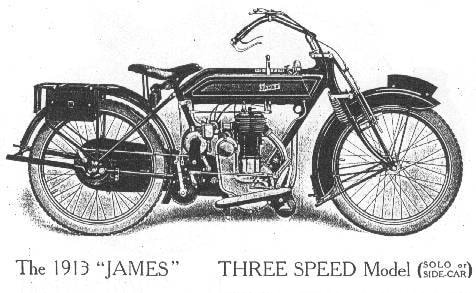
\includegraphics[width=1\textwidth]{figures/James1913}
     \caption{Advertisement for the 1913 James motorcycle}
     \label{fig:James}
\end{figure}

\begin{figure}[p]
	\centering
     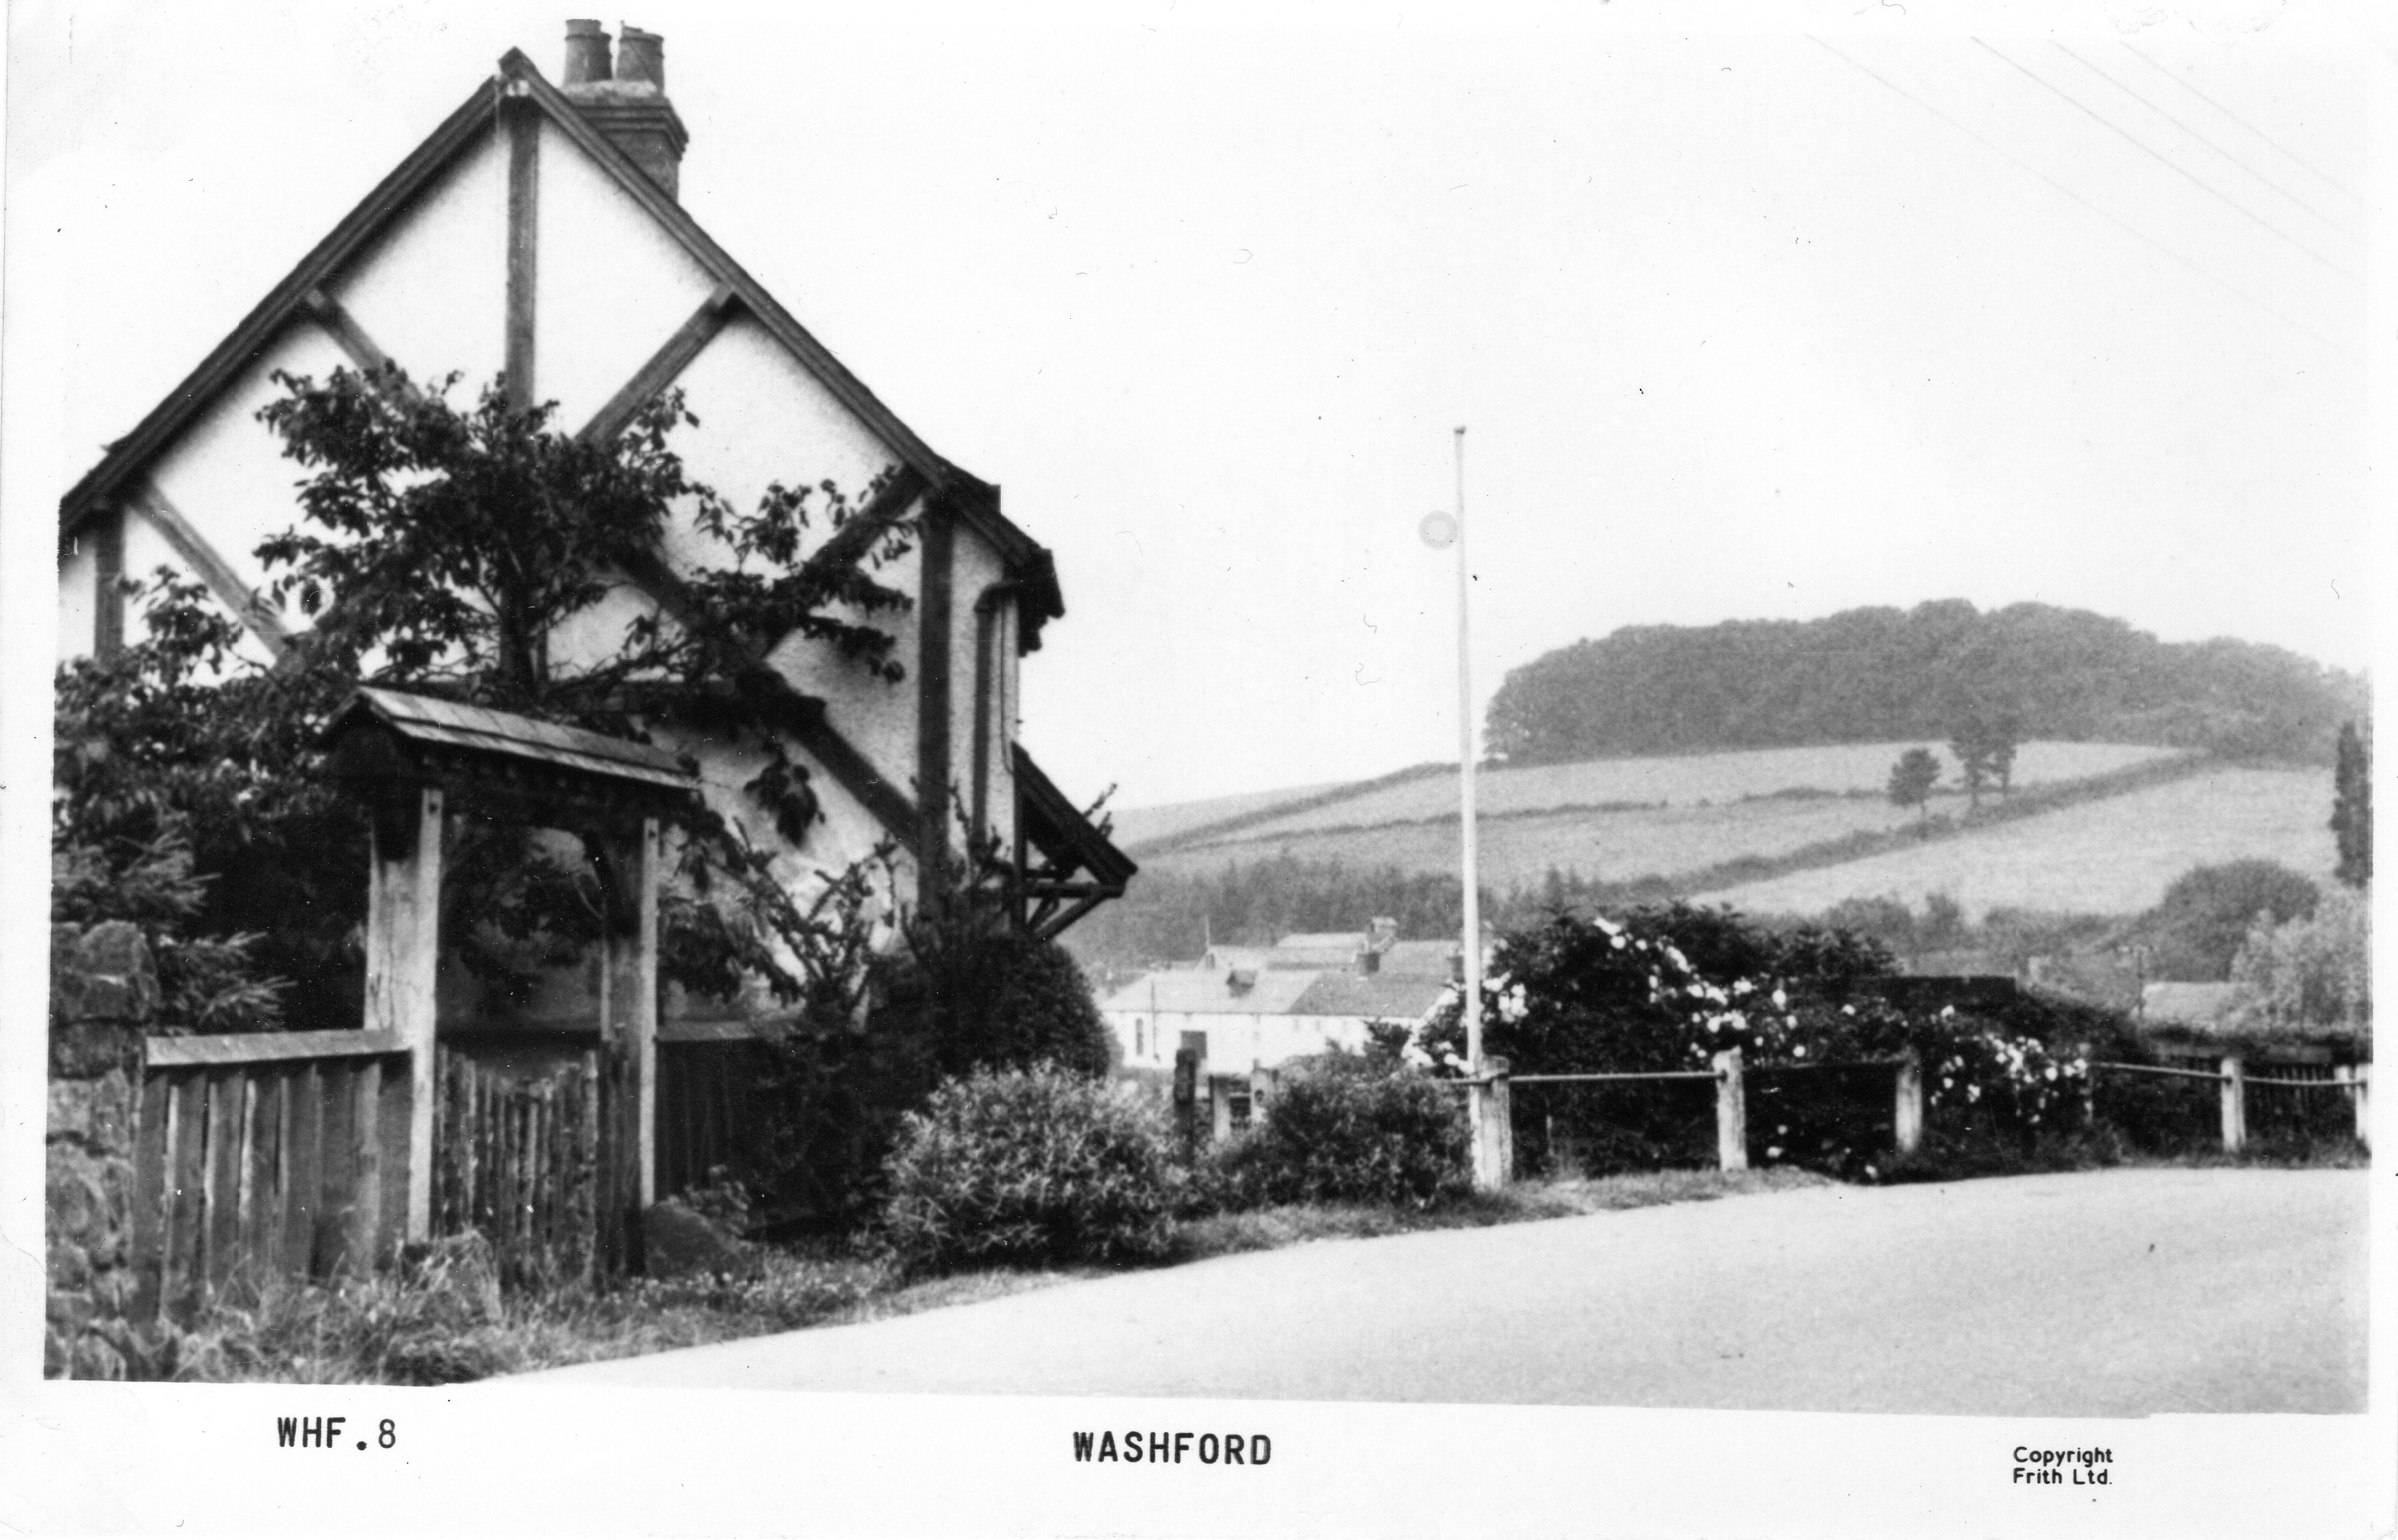
\includegraphics[width=1\textwidth]{figures/Postcard}
     \caption{The front entrance to Hill Head House and the neighbouring cottage, 1935}
     \label{fig:Postcard}
\end{figure}

\afterpage{\clearpage}

That must surely be all the re-usable material which as far as we can deduce found its way into various parts of the garden - but perhaps not quite all even now. Right at the back of the garage we found a heap of old tiles from Victorian fireplaces - of various designs and in lowering degrees of crudity as far as colour was concerned. The best ones were a deep olive green or burgundy red. The worst had bouquets of orange and purple flowers - William Morris gone wrong. The tiles are well over a quarter of an inch thick and the glaze nearly as thick as a sheet of glass. It seems very likely that some of them came from the cottages. We found a use for some of them when converting the wash house into a holiday chalet -they fitted the window ledge perfectly and it gave us great satisfaction to fit them into place and finish off the window so pleasantly and usefully.

In fact one of the most enjoyable aspects of living in a place like ours, now that after eight years the worst of the confusion has been sorted out, is to re-use some of the things that have been lying about for so long. I have been fortunate in finding a handyman who also enjoys this sort of thing and it becomes quite a game to find what we need somewhere on the premises. For example, we needed a brass door knob when tidying up; the door of the outside toilet - we knew we had seen one lying about somewhere, and on duly searching for it two were found! Pieces of wire and odd lengths of wood of course are always to be had. A year or two ago gypsies called one day and persuaded us to part with a lot of old telephone wires and scrap metal. I was glad to see it go but could not help wondering how	much the lead in the wire was worth. Our neighbours know that they can always come and ask us if they need a few pieces of wood for knocking up a rabbit hutch or fruit cage.

Last but not least I must not forget the window frames. They were rather small and old, so that even William found it difficult to find a use for them. They are still with us and it seems unlikely that they will ever be used. Some of them found their way into the back wall of the garage where a student of the subject will readily observe a veritable patchwork of lights serving the dual purpose of usefulness and economy: useful, as they let light in for seeing into the back of the garage, and economical, as they presumably proved to be a cheaper way of constructing a wall than purchasing yet more corrugated iron!
